\documentclass[border=12pt]{standalone}
\usepackage{tikz}
\usetikzlibrary{shapes.geometric, arrows.meta, positioning, calc, fit, backgrounds}
\usepackage{fontspec}
\usepackage{amsmath,amssymb}
\setmainfont{DejaVu Sans}

\begin{document}
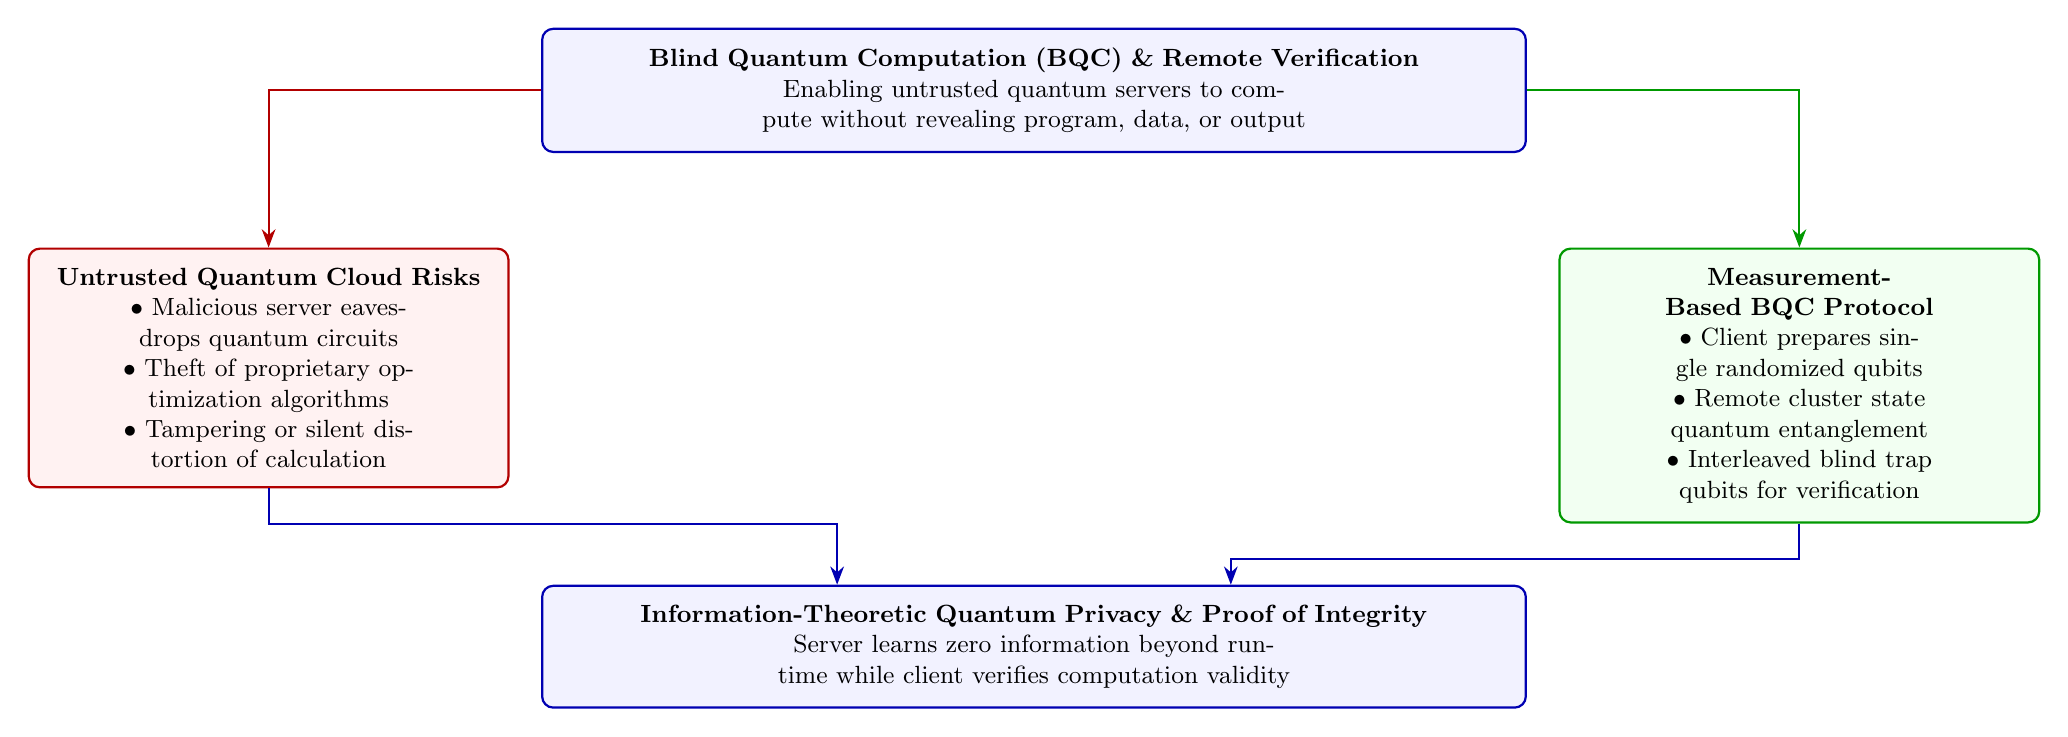
\begin{tikzpicture}[
    font=\small,
    >=Stealth,
    node distance=1.2cm,
    block/.style={rectangle, draw=blue!70!black, fill=blue!5, rounded corners=4pt, thick, align=center, inner sep=7pt},
    alertblock/.style={rectangle, draw=red!70!black, fill=red!5, rounded corners=4pt, thick, align=center, inner sep=7pt},
    greenblock/.style={rectangle, draw=green!60!black, fill=green!5, rounded corners=4pt, thick, align=center, inner sep=7pt},
    amberblock/.style={rectangle, draw=orange!80!black, fill=orange!5, rounded corners=4pt, thick, align=center, inner sep=7pt}
]

\node[block, text width=12cm] (top) {\textbf{Blind Quantum Computation (BQC) \& Remote Verification}\\Enabling untrusted quantum servers to compute without revealing program, data, or output};

\node[alertblock, below left=1.2cm and 0.4cm of top, text width=5.6cm] (server_threat) {\textbf{Untrusted Quantum Cloud Risks}\\$\bullet$ Malicious server eavesdrops quantum circuits\\$\bullet$ Theft of proprietary optimization algorithms\\$\bullet$ Tampering or silent distortion of calculation};

\node[greenblock, below right=1.2cm and 0.4cm of top, text width=5.6cm] (bqc_mbqc) {\textbf{Measurement-Based BQC Protocol}\\$\bullet$ Client prepares single randomized qubits\\$\bullet$ Remote cluster state quantum entanglement\\$\bullet$ Interleaved blind trap qubits for verification};

\node[block, below=1.0cm of $(server_threat.south)!0.5!(bqc_mbqc.south)$, text width=12cm] (bottom) {\textbf{Information-Theoretic Quantum Privacy \& Proof of Integrity}\\Server learns zero information beyond runtime while client verifies computation validity};

\draw[->, thick, red!70!black] (top) -| (server_threat);
\draw[->, thick, green!60!black] (top) -| (bqc_mbqc);
\draw[->, thick, blue!70!black] (server_threat.south) -- ++(0,-0.45) -| ([xshift=-2.5cm]bottom.north);
\draw[->, thick, blue!70!black] (bqc_mbqc.south) -- ++(0,-0.45) -| ([xshift=2.5cm]bottom.north);

\end{tikzpicture}
\end{document}
